\documentclass{article}
\usepackage{hyperref}
\usepackage{graphics}

\bibliographystyle{plain}
\begin{document}
\title{Birch: A Metadata File System}
\author{Casey Marshall \\
  University of California, Santa Cruz \\
  CMPS 221: Advanced Operating Systems\footnote{This work was done in
    fulfillment of the project requirements for the UCSC graduate
    course CMPS 221, Advanced Operating Systems, professor Scott
    Brandt, Fall 2006.} \\
  \texttt{csm@soe.ucsc.edu}}
\maketitle

\begin{abstract}
  We preset a dynamic file system for Mac OS X that renders metadata
  search results as files and directories, and describe the issues
  that arose in developing this system, and the lessons learned about
  the usability and performance of such a system.
\end{abstract}

\section{Introduction}
The advent of computers into our lives has brought a mixture of both
endless possibility and intense confusion. While we now have the
ability to store and use a myriad of different file types for anything
we may need --- text files, images, videos, music, each with dozens of
file formats --- our ability to manage and find things we need has
gone down as the number of files we use goes up. The common way
computer users organize media is through a hierarchical file system,
that stores data (files) in lists (directories); the file system is,
then, a list of lists, forming a rooted tree. This model is an
excellent, simple way to organize data, and it has served computer
users well. The issue with hierarchical file storage is that it
depends on the user to create and manage these hierarchies, and so the
quality and usability of a particular hierarchy is only as good as the
effort put into defining that hierarchy. Good classification schemes
are difficult for the average computer user to define --- we have
historically relied on professionals to organize large collections of
data. Furthermore, some data may simply defy hierarchical
classification, and can fit into many different taxonomies.

These limitations of hierarchical file systems have been expounded
upon by many others \cite{OToole:1992, Nielsen:1996, Gorter:2004,
  Nickell:2006}, and yet, few alternatives seem to gain traction in
wide use.  We, along with others~\cite{Veda:2005}, think that new,
better information-centric interfaces will appear in future computer
systems.

Birch is an experimental file system that uses a simple
model --- directories are queries, files are matches to queries, and a
path of directories forms a conjunction --- to push an alternative
data organization into the file system. Birch uses an existing
metadata search system, Spotlight, and renders Spotlight metadata
searches as a file system.

We don't consider Birch a success in its present form; a combination
of the quality of searches possible, and the difficulties in making a
highly dynamic system operate when serving highly synchronous I/O
primitives make it a far cry from usable. Some of these issues are
undoubtedly due to our simple definitions of directories and files,
and some are because of the short development time --- about two
months, part time.

%Birch is named after the trees outside the author's window, and is
%ironic, since it names something that tries to do away with trees
%after a kind of tree.

\section{Related Work}

We have already seen alternative interfaces in client applications
that access certain kinds of computer files in a non-hierarchical way:
Apple's iTunes accesses music and video files based on content, and
through play lists the user can create and edit. The Finder
application supports so-called ``smart folders,'' which use the
Spotlight metadata service to display a simple metadata query as a
folder. All of these are useful, but are orthogonal to one another ---
groupings made in one application cannot be used in other
applications.

There have been efforts to provide similar, general-purpose user
interfaces --- a database file system, as an alternative file manager
and graphical shell for the GNOME and KDE desktop
environments~\cite{Gorter:2004}. This database file system solves much
of the problem of application-specific searches by augmenting the file
dialogs that GNOME and KDE programs use, when a person opens or saves
a file in an application. Metadata queries and arbitrary groupings are
made global at the UI interaction level. The Haystack
project~\cite{Karger:2003} is a loose collection of applications that
present new ways of working with semi-structured data.

The semantic file system \cite{Gifford:1991} closely resembles Birch,
both in goal and in function. In the semantic file system, special
directory names are used to form queries by referencing
``transducers,'' which match files against various criteria.

Tagging, in which users add keyword-style categorizations of files, is
extremely popular in recent web sites such as Flickr and delicious,
and can form ad-hoc user-generated taxonomies \cite{Mathes:2004}. Tags
are put into use in the TagFS system \cite{Bloehdorn:2006}.

The Spotlight system built in to Mac OS X, starting with version 10.4,
provides a rich language for interacting with various file
attributes. Spotlight uses a key-value mechanism, where a metadata key
--- for example, \texttt{kMDItemFSName}, which is the key for the
file's name --- is mapped to a value for each file. Metadata keys can
reflect file system information, such as the file's name or modified
time, or they can be \textit{content-based,} giving a richer overview
of the file's content; this can include anything from a list of
authors, to the bit rate for digital video and audio, to the color
space of digital images. Files that don't have a sensible metadata
value for a given key have a nil result for that key. Spotlight is the
metadata system we use in Birch, and we find it usable, if lacking in
quality in some areas.

\section{File System Concepts}

\subsection{Why a Stacking File System}

We could implement our alternative file access system purely in a
client application, similar to the existing Finder application, and
some existing efforts \cite{Gorter:2004,Nickell:2006} work from this
model. We do, however, have an existing wealth of applications that
use the standard C library calls \texttt{open}, \texttt{read},
\texttt{write}, etc. Presenting new views of data through a file
system allows us to use existing programs to access these data,
without modifying the underlying program. This idea is a powerful one,
and is not new --- the design of the GNU Hurd \cite{Bushnell:1994}
emphasizes the power of this idea, and new APIs such as FUSE
\cite{Szeredi:2006} bring this idea to other operating systems.

\subsection{Directories as Sets}

The key concept in our file system design is that a directory
represents a \emph{set:} an unordered collection of unique files, and
any particular file may exist in multiple sets. This definition
doesn't stray very far from the formal definition of a directory ---
which is a list of files and subdirectories. The difference between
directories and directory-sets is that sets are not necessarily part
of a rooted hierarchy, and can instead be composed with one another in
arbitrary ways.

Subdirectories, and paths, define a path through the rooted file tree
to a specific file, using the character \texttt{/} to separate
components. Thus, \url{/Users/csm/file.txt} defines a path through
the file system tree that identifies a file \texttt{file.txt}. With
directory-sets, the \texttt{/} character becomes a \emph{conjunction
  operator,} and so the path of directories becomes an intersection of
all named sets in the path. Thus, if we have two named sets
\texttt{foo} and \texttt{bar}, each of which has some number of files,
some of which may be common, the path \texttt{foo/bar} (or
\texttt{bar/foo}) contains the intersection of files in \texttt{foo}
and the files in \texttt{bar}. The union of two sets can be gotten by
reading the contents of one set, then the next, then removing
duplicates; in other words, \texttt{ls foo bar | sort | uniq} would
produce an accurate union of two sets \texttt{foo} and \texttt{bar}.

\subsection{Directories as Predicates}

Managing the file system using sets, whose contents may be completely
arbitrary, is a fine notion in itself; what we lack then, is a way to
define these sets. We can imagine this being done by hand: copying, or
perhaps linking, a file from one set into another places the file in
both sets. Limiting ourselves to simple POSIX file system operations
makes this kind of management difficult and error-prone. If we were to
try to maintain set semantics given the low-level file I/O functions,
the system would quickly collapse.

An alternative is having every directory represent a predicate --- a
simple metadata query, such as ``name equals `foo'.'' That is, an
assertion about a file's attributes that has a boolean result; such a
predicate, when tested on a collection of files, defines a set. The
intersection of two sets is then defined as the conjunction of the two
directory-sets' predicates. There is currently no explicit way to
define a disjunction of two or more predicates, but this may be a
future extension to the system: wherein each directory-set represents
a disjunction of one or more metadata assertions, and path composition
forms the conjunction of statements, as above. This is the conjunctive
normal form, assuming that each predicate operator has an inverted
companion, and thus it is of sufficient power to express any query.

\subsection{Naming}

In order to reference an existing set when building a path, our system
requires that set names are global. This has some obvious drawbacks,
since it replaces, in the user's experience, a hierarchical naming
burden --- the burden of organizing files in a sensible directory
hierarchy --- into a flat naming burden --- that of coming up with a
unique name for each query.

This is not as bad as it sounds. Since queries are inherently more
powerful than directories, and because they are reusable in many
places, there should be fewer queries than directories. Query names
can be evocative of their function, so the query named ``Author is
Brian Eno'' would be a query that looked for files where the
``author'' is Brian Eno. It is still up to the person using the system
to invent a good name for a query, but naming queries can be simple,
if the name is evocative of the function.

\section{Implementation}

Birch is implemented as a Cocoa application that creates a user-space
NFS system, and NFS RPC calls (which only come over a local socket
instead of over the network) are interpreted to render metadata search
queries as files and directories. A simple Cocoa user interface (shown
in figure~\ref{figure:mainwindow}) manages the search queries the
file system renders. Queries are composed using the
\texttt{NSPredicate} and \texttt{NSMetadataQuery} classes, which
access the Spotlight metadata database.

\begin{figure}[ht!]
  \begin{center}
    \scalebox{.5}{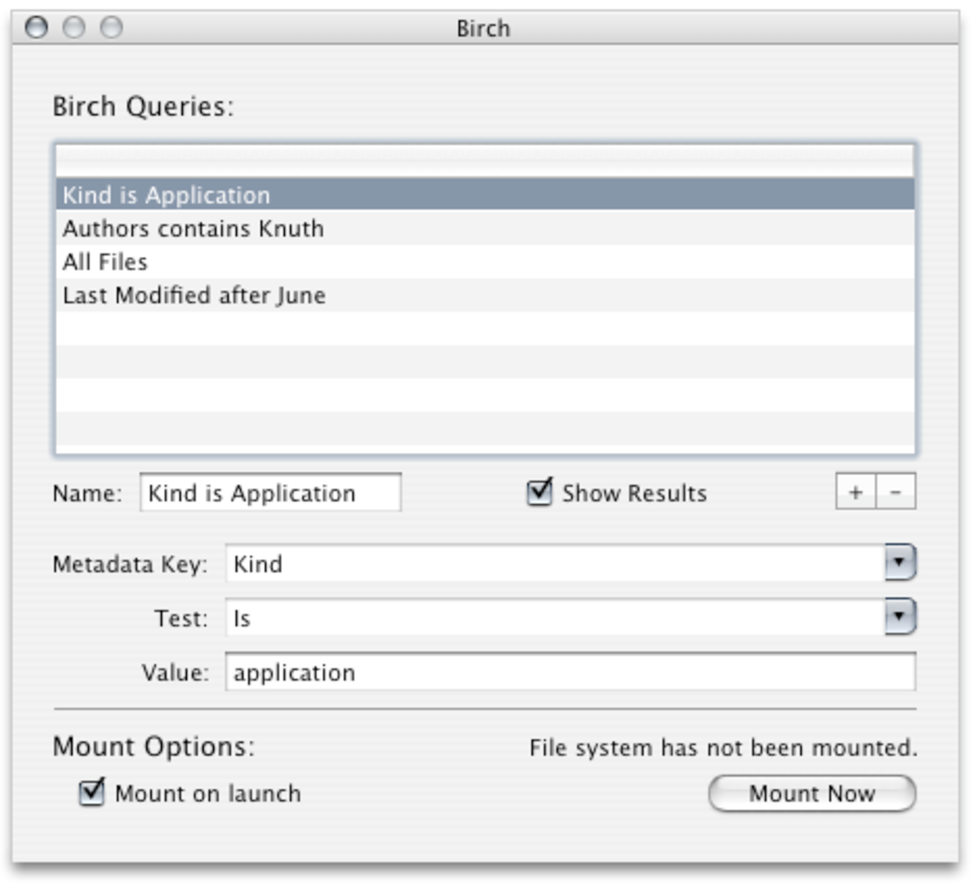
\includegraphics{birch-control}}
    \caption{The Birch control interface.}
    \label{figure:mainwindow}
  \end{center}
\end{figure}

The basic object is the system is the Query, which contains three
fields:

\begin{itemize}
\item The \emph{predicate,} which is a Spotlight query stored in an
  \texttt{NSPredicate} object. An example query is
  \texttt{"kMDItemAuthors == '*Brian Eno*'"}.

\item A boolean attribute \emph{isLeaf.} ``Leaf'' queries show their
  results in the file system view; non-leaf queries do not. The
  purpose of non-leaf queries is to store a partial query, which can
  be composed with other queries. Since the partial query may match
  too many files, the non-leaf attribute prevents large, possibly
  uninteresting, result sets from being displayed.

\item A set of names of other sets, called \emph{subordinates.}
  Subordinate sets are always shown in the file system, and provide a
  way to save metadata search paths. For example, one could store a
  query, like \texttt{"kMDItemAlbum == '*Music for Airports*'"}, inside
  a query that it is commonly used with, such as
  \texttt{"kMDItemAuthors == '*Brian Eno*'"}. There is no hierarchy
  implied here; two queries may contain one another in their
  subordinate sets, and conjunctions can be formed by specifying
  either one first.

  This provision is a concession that some ways that people access
  files doesn't allow them to type in (or even remember) the names of
  queries. For example, we can type the name of any set when using the
  shell, but in Finder, for example, we get a graphical display of the
  working directory, and while a user could use the ``New Folder''
  command, giving the new folder the name of the query, having them
  immediately available is friendlier.
\end{itemize}

Each query also has a name, which must be unique amongst all other
query names. A request for a path, say \texttt{/Kind is PDF/Authors
  contains Knuth/}, where the query named ``Kind is PDF'' corresponds
to the predicate \texttt{kMDItemKind == 'PDF'}, and the query named
``Authors contains Knuth'' corresponds to the predicate
\texttt{kMDItemAuthors == '*Knuth*'}, the compound predicate for the
path would be \texttt{kMDItemKind == 'PDF Document' \&\&
  kMDItemAuthors == '*Knuth*'}. If either query has its
\textit{isLeaf} attribute set to true, then the path will display all
results that match the conjunction.

In order to simplify the implementation of the NFS server, no file I/O
requests are handled by the NFS server itself. Instead, files
referenced in a query always appear as symbolic links, where the
content of the link is the full path to the file elsewhere on the file
system. This mechanism greatly simplifies the objects the Birch file
system needs to keep track of: everything in the file system is either
a directory, and thus a predicate, or it is a link to a file matching
a predicate. We think this kind of file system --- which only uses
links to reference resources --- is a very useful implementation
strategy, since it simplifies and optimizes file access, once the file
is looked up. This makes the file system analogous to other forms of
search results, like Internet search engines, which produce as output
not the content found, but merely links to the content. It is also
much easier to properly implement POSIX semantics if the capabilities
of the file system are restricted, which was invaluable given the
short development time of this project.

There are four ``kinds'' of metadata supported by Birch, and each kind
supports different tests. The kinds of metadata available for search
are~\cite{appleref:spotlight-metadata}:

\begin{itemize}
  \item\textbf{Strings}. Valid tests include equality, inequality,
    starts with, ends with, and contains. The operand of the test may
    be any string.

  \item\textbf{Dates}. Valid tests are equality, inequality, before
    date, and after date.

  \item\textbf{Numbers}. Valid tests are equality, inequality, less
    than, and greater than.

  \item\textbf{Arrays of strings.} Valid tests are contains, and does
    not contain. Containment is, in spotlight queries, equivalent to a
    substring match in the concatenated list.
\end{itemize}

The root directory of the file system is a pseudo-query itself, which
matches all files, is not a leaf, and contains all other queries as
subordinates. Thus, the root directory shows a view of all other
queries. Creating a new directory in any directory will do one of two
things: if the new directory is named the same as an existing query,
then that query is placed into the containing query's subordinate set,
and from then on can be accessed to form a conjunction with the
containing query; if the name is new, a new query is created in the
database, which has a null predicate (i.e., it matches anything), is
not a leaf query, and has no subordinates. That query can then be
modified through the Birch user interface.

\subsection{Lookups and Caching}

In the NFS protocol, version 2, a ``file handle'' --- an opaque
identifier used by NFS clients to identify files that have been looked
up --- is 32 bytes long. In Birch, a file handle is always composed by
using the MD5 \cite{RFC1321} checksum of the file's path, with the
upper 16 bytes padded with zero. The only exception is the root file
handle, which is always 32 zero bytes, and the root path always begins
with the string \texttt{"/Birch"}. Thus, a virtual path
\texttt{"/Birch/foo/bar"} will have the file handle

\begin{center}
  \texttt{2c804fc3 5adb5c62 96f46043 b1a09cec} \\
  \texttt{00000000 00000000 00000000 00000000}
\end{center}

\noindent These file handles are mapped internally to directory entry
(``dentry'') structures, which track the kind of file, the file's
name, its parent dentry, and so on. We can thus build the full path of
any dentry by walking up the list of parent dentries, and thus we can
reconstruct a file handle if we are only given a parent directory file
handle and a file name --- we just compute the MD5 hash of the parent
file path concatenated with the file name. Thus, the NFSv2
\texttt{LOOKUP} command can quite quickly look up a file by name,
given its parent directory's file handle, using only two hashtable
lookups, one string concatenation, and one MD5 computation.

In order to support certain core OS X applications like the Finder
better, Birch does support memory-only read/write files, for things
such as the \texttt{.DS\_Store} file (which Finder uses to store
window state information). Birch also always contains an empty,
non-modifiable file \texttt{.metadata\_never\_index} in every
directory, which prevents Spotlight from indexing the mounted Birch
file system.

\section{Interpretations and Limitations}

\subsection{Metadata Quality and Availability}

Birch uses the Spotlight database for its metadata searches, mostly
out of convenience, since this database exists on, and is constantly
updated by, Mac OS X by default. We have found Spotlight to be less
than ideal for robust, usable searching, and efforts to improve
metadata indexing would benefit Birch, and Spotlight users in
general. The problem with Spotlight is that it imports metadata keys
(other than the obvious ones, available through the file system for
all files) via ``tagged'' content. Many file formats --- AAC or MP3
audio, PDF documents, video formats, etc. --- support metadata
``tags,'' or key-value pairs that describe the content. Spotlight uses
this information, where it is available, to populate its database ---
so if an AAC file is tagged with artist ``Bob Dylan,'' Spotlight can
populate the \texttt{kMDItemAuthors} key with that info. If a file is
not tagged, or is tagged incorrectly, then a proper index cannot be
built.

One example of Spotlight's limitations is the ``authors'' key, when
applied to PDF files. Ideally, one should be able to find any PDF file
on a system --- say, if it was in a collection of academic papers ---
by searching for one of the authors. Many programs that produce PDF
output don't tag the document with this information, of if it does, it
requires that the creator fill in these fields manually, meaning that
most of the time this meta-information is omitted. This is a general
problem when doing content-based indexing.

\subsection{Leaves are more sparse than internal nodes}

A set-based file system like we have presented here necessarily, and
literally, turns the file system hierarchy on its head: since a leaf
node is defined as a series of conjunctions, leaves are always more
sparse than nodes higher up in the tree. This can be a usability
problem, since a person using the file system would, in general, be
presented with more files early on in her browsing, and may be
overwhelmed with the number of files present so high up in the tree.

There are potential refinements we can make, to help alleviate this
scenario: one could be to make the subdirectory relationship a
disjunction, instead of a conjunction, and make each directory
predicate a conjunction of assertions. This would make the file system
layout more ``tree-like,'' while retaining the power of a full logical
language (the disjunctive normal form).

Another alternative would be to make all query directories non-leaf
--- that is, make them so they never show their results --- and then
in each directory present a pseudo-directory called ``results,'' which
``leafifies'' the parent statement. This way, a person is never
overwhelmed by intermediate results: she either is browsing through
available queries, or is inspecting the results of a query.

We recognize, too, that these issues stem directly from our insistence
on making the file system have POSIX semantics; without that
requirement, and the tree structure it implies, a new interface may,
in fact, be better. Using POSIX semantics is valuable when working
with existing programs, but may pose barriers to usability.

\subsection{Getting Lost}

Because directory names are global, it is easy to get ``lost'' while
browsing the file system: the person browsing has no indication that
the directory he is in is deep or not. That is, it is very hard to
tell if a query has a parent query (which, if it does, will produce a
conjunction) and thus opening a particular directory may give
unexpected results.

\subsection{Synchrony}

A significant problem with Birch is how it interacts with synchronous
I/O operations --- in some early versions of the program, metadata
queries took so long to produce any results, even if those results
returned a nil result set, that the OS X NFS client timed
out. Applications like Finder are completely unresponsive while some
I/O operations, like \texttt{readdir}, are taking place. A complicated
query with few results can render some applications unusable for
minutes at a time.

We have taken some measures to improve this, such as adding an
internal timeout for metadata queries, such that if the query produces
no new results within 5 seconds, we end the query with the partial
results. This is of only moderate help, of course, because the
application will remain unresponsive for at least 5 seconds, or
longer, if incremental updates to the result set happens every five
seconds.

Another issue is with queries that match many, many files. These can
produce directories that contain hundreds of thousands of files, and
again, some applications are unresponsive until \emph{all} files have
been read out of a directory. A simple workaround that we use here is
a hard cap of 10,000 files per directory. This is not a robust
solution, but we see no other way of forcing large queries to finish
in a reasonable amount of time.

We are unsure if this limitation is inherent in the POSIX API and ---
more importantly --- applications that use that API, or a limitation
in NFS version 2 and the client-side support built into OS X. We don't
see any way to force applications to update with partial results,
while still polling the directory --- many applications simply insist
on reading an entire directory before returning any results.

Modern operating systems like Mac OS X also have some form of event
notification, that notifies listeners when operations on files are
performed. The Linux kernel has the \texttt{inotify}
mechanism~\cite{Dow:2005}; Microsoft Windows NT, 2000, and XP have the
\texttt{System.IO.FileSystemWatcher}
class~\cite{MSDN:FileSystemWatcher}; Mac OS X has, in 10.4 and with a
public API in 10.5, the \texttt{fsevents} mechanism. Each of these
notifies listeners of various events that happen to the local file
systems, such as when files are created, removed, modified, etc. Since
Birch uses a NFS server to implement the file system in user space, it
cannot notify the kernel of events that happen in the virtual file
system, such as a new match to one of the queries. Having a mechanism
where Birch could notify the kernel of events would help solve the
issue with blocking during \texttt{readdir}: the system only lists
files it matches immediately, and from then on posts the remaining
search results as events.

\subsection{Forming Conjunctions}

As we have mentioned, a directory path forms a conjunction of all
predicates in that path. The implementation of this simply forms a new
\texttt{NSPredicate} with all of the terms joined with the conjunction
operator, \texttt{\&\&}. Running complicated queries with many terms
is relatively slow; this can, in principle, be optimized by using the
results from the partial query and running the additional terms on
successive partial results.

\subsection{File Lookups, Caching, and Consistency}

When a client performs a \texttt{readdir}, all matched files are
inserted into the dentry cache, so when the client comes back to
\texttt{lookup} each of these, we will have the entries ready. If a
file is not in the dentry cache, we are left with the problem of
looking up a file, which both matches a query (defined by the
containing directory) \emph{and} the requested file name. This is
simple enough to define, by forming a conjunction of the query and a
term that matches \texttt{kMDItemFSName}. This kind of query is very
slow, especially if it fails to match any files; our only recourse, to
maintain responsiveness, is to only run these queries briefly,
returning \texttt{ENOENT} if nothing is found.

This caching strategy works well to avoid this issue: after a
\texttt{readdir}, chances are that any file that will be looked up
will exist in the dentry cache. We then, however, have a problem with
when to expire dentry cache entries: flushing them early will mean
that subsequent \texttt{lookup} calls will likely fail. Not flushing
old entries, or flushing them rarely, from the cache is a memory
burden, and the system will not scale. Also, since the dentry cache
can be extremely large, removing the least-recently-used entries (the
cache is an associative map from file handle to directory entry) is
time-consuming.

\subsection{Usability}

Our goal when starting this project was to investigate a different,
and hopefully better, way of presenting files to people using the
system. While we think there is value in search-based systems, as well
as presenting these search results in a file system interface,
navigation of the present implementation is difficult, both because of
the technical limitations --- the slowness of the system in executing
large queries, and issues with programs interacting with slow system
calls --- and the confusion that undoubtedly takes over someone
navigating a new, alien conceptual space as presented here: we can't
expect the average person to understand metadata searches and
conjunctions.

A ripe area for more investigation is improving the interface for
defining and editing metadata queries. We like, for example, the
interface that Mac OS X has for defining ``smart folders'' ---
what is missing is presenting these searches as a file system.
Simplicity may be a benefit here; Internet search engines are largely
so effective because of their simple interface: a list of keywords
with a simple syntax for defining phrases is sufficient for a wide
variety of searches.

\section{Performance Measurements}

In this test we chose to run some ``primed'' metadata queries --- that
is, we ran the query once before running the test, to ensure that the
metadata server can cache that query --- using both \texttt{mdfind}
(the command-line interface to Spotlight) and \texttt{ls -l} on a
mounted Birch file system. These tests were run on a MacBook Pro with
a 1.83GHz Intel Core Duo, and 1GB of RAM. The system has a single 80GB
SATA hard disk about two thirds full with the author's files. The
results of these runs are presented in figure~\ref{fig:benchmarks}.

\begin{figure}[ht!]
\begin{center}
\begin{tabular}{|l|c|c|r|} \hline
 \textbf{Query} & \texttt{mdfind}   & \texttt{ls -l} & \textbf{result count} \\ \hline \hline
\texttt{kMDItemKind == Application} & 0:00.688 & 0:02.043 &   216 \\ \hline
\texttt{kMDItemFSName == *.txt}     & 0:20.090 & 0:22.701 &  1146 \\ \hline
\texttt{kMDItemFSSize > 1024 \&\&}  & 2:12.543 & 2:48.835 & 12655 \\
\texttt{kMDItemFSSize < 1280}       &          &          &       \\ \hline
\texttt{kMDItemFSSize > 1024 \&\&}  & 2:08.499 & 2:06.944 &    39 \\
\texttt{kMDItemFSSize < 1280 \&\&}  &          &          &       \\ 
\texttt{kMDItemFSName == *.txt}     &          &          &       \\ \hline
\texttt{kMDItemKind == *Image*}     & 0:01.111 & 0:30.731 &  6010 \\ \hline
\texttt{kMDItemNumberOfPages == 12} & 0:00.545 & 0:00.668 &     5 \\ \hline
\end{tabular}
\caption{Query benchmarks}
\label{fig:benchmarks}
\end{center}
\end{figure}

These results seem to show that the bulk of the time spent in the file
system is running the query, and that the NFS protocol overhead (which
includes a \texttt{lookup}, \texttt{getattr}, and \texttt{readlink}
call for every search result, along with the \texttt{readdir} calls)
is low. An excellent refinement to Birch is to run queries in the
background, caching the results until a client arrives to read
them. The numbers also indicate that complicated queries that use
wildcard patterns, have many terms, or read certain attributes take
longer to run.

\section{Conclusion}

We have presented a prototype file system that renders search queries
as files and directories. We have some technical hurdles left to
overcome, especially in the area of performance, given that many
applications are reading dynamic, asynchronous results with a highly
synchronous API. The Spotlight metadata service is useful in this
project because it already exists, and provides a number of
interesting fields to search, but is in our opinion too limited in the
quality of searches, and it performs too poorly to become a core part
of the system's I/O.

In the course of developing this project, we uncovered a bug in the OS
X NFS client support, which resides in the kernel. An early version of
Birch was able to cause a kernel panic, simply by returning malformed
NFS RPC replies.

\bibliography{Sources}

\vfill
\begin{center}
  \scalebox{.25}{
\includegraphics{birch-tree.png}} %\\
%  {\small The name ``Birch'' merely comes from the \\
%   kind of trees outside the author's window, \\
%  and is meant to be ironic, since the Birch \\
%  file system \emph{subverts} tree-based layouts.}
\end{center}
\vfill

\end{document}
